\section{Framework Design}

\begin{concept}{Framework Grundlagen}\\
Ein Framework ist ein Programmiergerüst mit folgenden Eigenschaften:
\begin{itemize}
    \item Bietet wiederverwendbare Funktionalität
    \item Definiert Erweiterungs- und Anpassungspunkte
    \item Verwendet Design Patterns
    \item Enthält keinen applikationsspezifischen Code
    \item Gibt Rahmen für anwendungsspezifischen Code vor
    \item Klassen arbeiten eng zusammen (vs. reine Bibliothek)
\end{itemize}
\end{concept}

\begin{definition}{Framework Entwicklung}\\
Die Entwicklung eines Frameworks erfordert:
\begin{itemize}
    \item Höhere Zuverlässigkeit als normale Software
    \item Tiefergehende Analyse der Erweiterungspunkte
    \item Hoher Architektur- und Designaufwand
    \item Sorgfältige Planung der Schnittstellen
\end{itemize}
\end{definition}

\begin{remark}{Kritische Betrachtung}\\
Herausforderungen beim Framework-Einsatz:
\begin{itemize}
    \item Frameworks tendieren zu wachsender Funktionalität
    \item Gefahr von inkonsistentem Design
    \item Funktionale Überschneidungen möglich
    \item Hoher Einarbeitungsaufwand
    \item Schwierige "Scheidung" nach Integration
    \item Trade-off zwischen Abhängigkeit und Nutzen
\end{itemize}
\end{remark}

\begin{KR}{Framework Design Principles}
\textbf{1. Abstraktionsebenen definieren}
\begin{itemize}
    \item \textbf{Core API:}
    \begin{itemize}
        \item Zentrale Interfaces
        \item Hauptfunktionalität
        \item Erweiterungspunkte
    \end{itemize}
    
    \item \textbf{Extensions:}
    \begin{itemize}
        \item Plugin-Mechanismen
        \item Callback-Interfaces
        \item Event-Systeme
    \end{itemize}
    
    \item \textbf{Implementierung:}
    \begin{itemize}
        \item Standard-Implementierungen
        \item Utility-Klassen
        \item Helper-Funktionen
    \end{itemize}
\end{itemize}

\textbf{2. Erweiterungsmechanismen}
\begin{itemize}
    \item \textbf{Interface-basiert:}
    \begin{itemize}
        \item Klare Verträge
        \item Lose Kopplung
        \item Einfache Erweiterung
    \end{itemize}
    
    \item \textbf{Annotations:}
    \begin{itemize}
        \item Deklarative Konfiguration
        \item Metadaten-getrieben
        \item Runtime-Processing
    \end{itemize}
    
    \item \textbf{Composition:}
    \begin{itemize}
        \item Plugin-System
        \item Service-Loader
        \item Dependency Injection
    \end{itemize}
\end{itemize}
\end{KR}

\begin{example2}{Prüfungsaufgabe: Framework-Analyse}
\textbf{Szenario:}
Ein Framework für die Verarbeitung verschiedener Dokumentformate (PDF, DOC, TXT) 
soll entwickelt werden.

\textbf{Aufgabe:}
Analysieren Sie die Design-Entscheidungen.

\textbf{Lösung:}
\begin{itemize}
    \item \textbf{Erweiterungspunkte:}
    \begin{itemize}
        \item Dokumenttyp-Erkennung
        \item Parser für Formate
        \item Konvertierungslogik
    \end{itemize}
    
    \item \textbf{Design Patterns:}
    \begin{itemize}
        \item Factory für Parser-Erzeugung
        \item Strategy für Verarbeitungsalgorithmen
        \item Template Method für Konvertierung
    \end{itemize}
    
    \item \textbf{Schnittstellen:}
    \begin{itemize}
        \item DocumentParser Interface
        \item ConversionStrategy Interface
        \item DocumentMetadata Klasse
    \end{itemize}
\end{itemize}
\end{example2}

\subsection{Design Patterns in Frameworks}

\begin{concept}{Abstract Factory}\\
\textbf{Problem:} Erzeugung verschiedener, zusammengehörender Objekte ohne Kenntnis konkreter Klassen\\
\textbf{Lösung:}
\begin{itemize}
    \item AbstractFactory-Interface definieren
    \item Pro Produkt eine create-Methode
    \item Konkrete Factories implementieren Interface
\end{itemize}
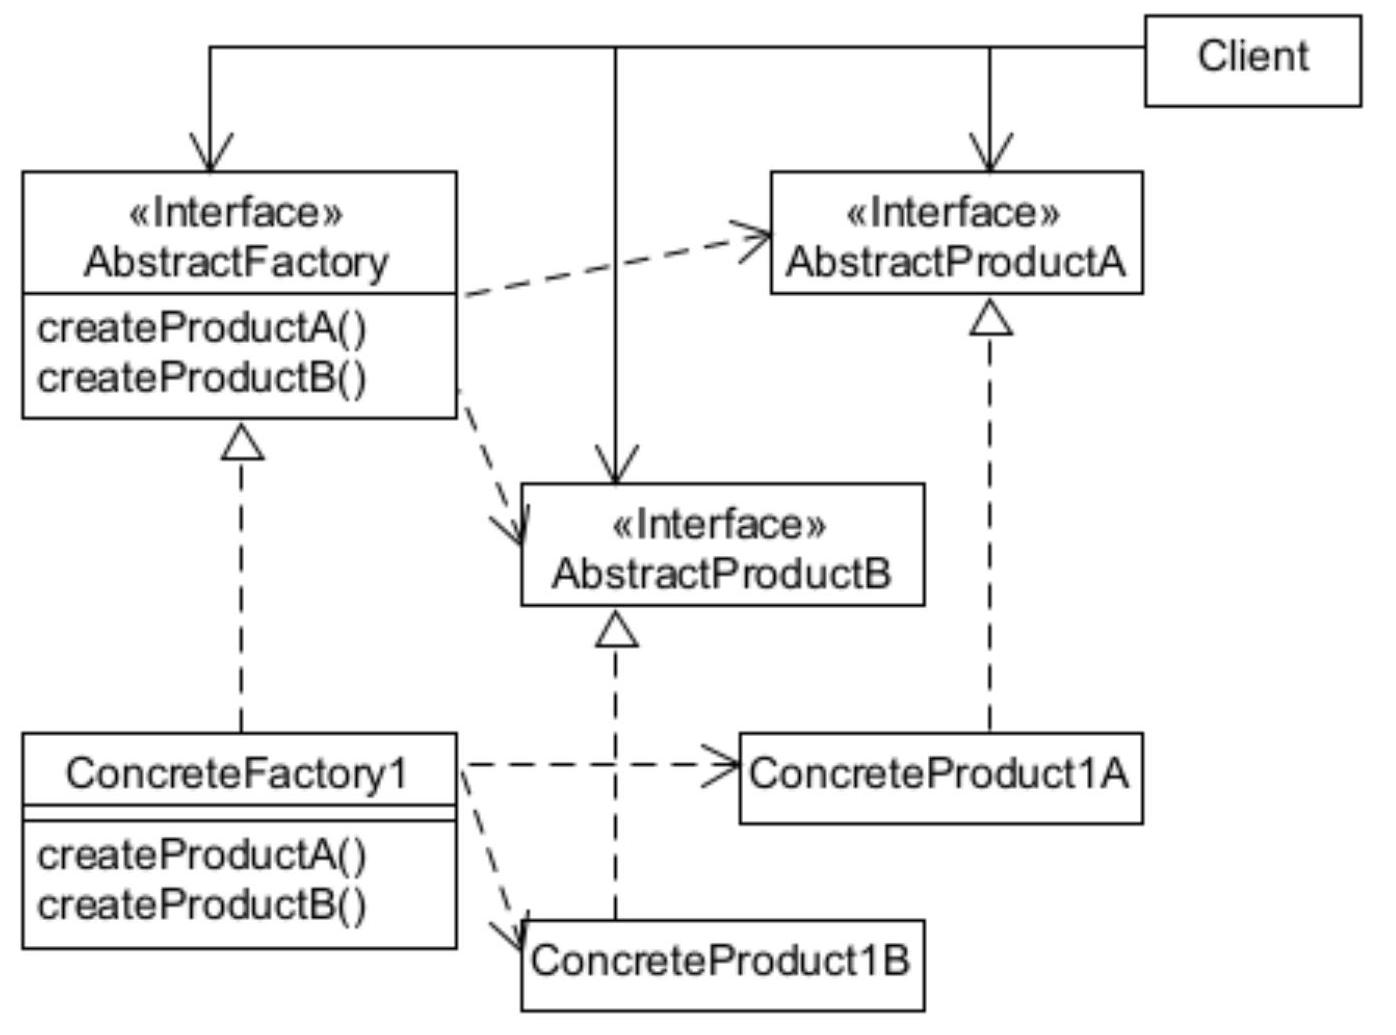
\includegraphics[width=0.8\linewidth]{images/2025_01_02_73d93f10fa91ab6123dcg-13}
\end{concept}



\begin{concept}{Factory Method}\\
\textbf{Problem:} Flexible Objekterzeugung in wiederverwendbarer Klasse\\
\textbf{Lösung:}
\begin{itemize}
    \item Abstrakte Factory-Methode in Creator-Klasse
    \item Konkrete Subklassen überschreiben Methode
    \item Parallele Vererbungshierarchien
\end{itemize}
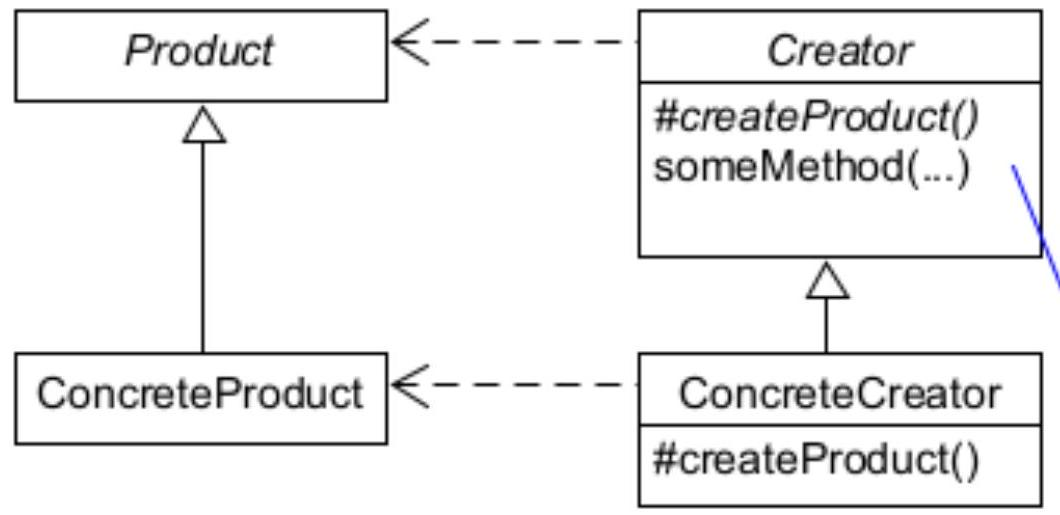
\includegraphics[width=0.8\linewidth]{images/2025_01_02_73d93f10fa91ab6123dcg-16}
\end{concept}

\begin{concept}{Command}\\
\textbf{Problem:} Aktionen für späteren Gebrauch speichern und verwalten\\
\textbf{Lösung:}
\begin{itemize}
    \item Command-Interface definieren
    \item Konkrete Commands implementieren
    \item Parameter für Ausführung speichern
    \item Optional: Undo-Funktionalität
\end{itemize}
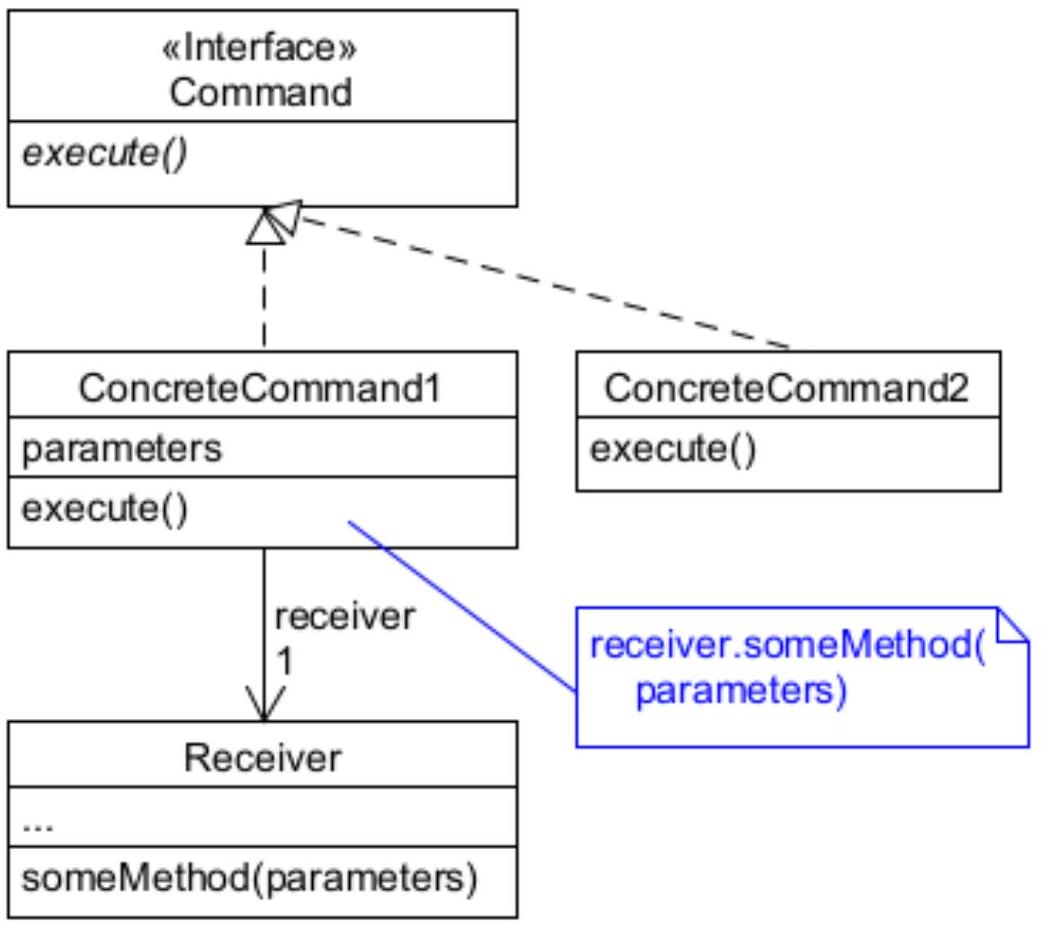
\includegraphics[width=0.8\linewidth]{images/2025_01_02_73d93f10fa91ab6123dcg-19}
\end{concept}



\begin{concept}{Template Method}\\
\textbf{Problem:} Algorithmus mit anpassbaren Teilschritten\\
\textbf{Lösung:}
\begin{itemize}
    \item Template Method in abstrakter Klasse
    \item Hook-Methoden für variable Teile
    \item Hollywood Principle: "Don't call us, we'll call you"
\end{itemize}
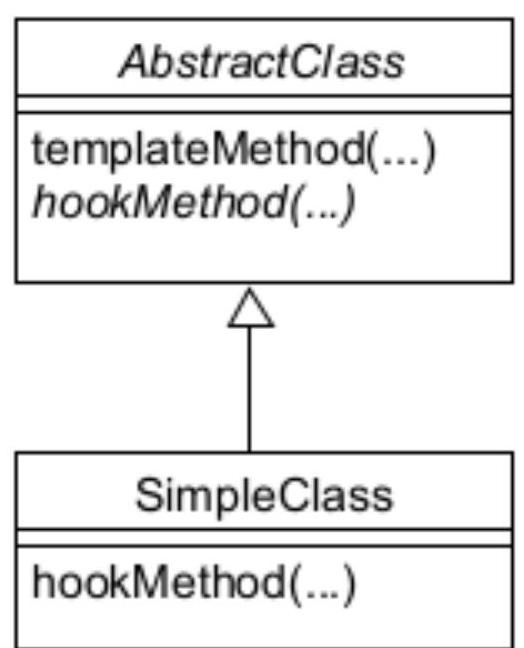
\includegraphics[width=0.8\linewidth]{images/2025_01_02_73d93f10fa91ab6123dcg-22}
\end{concept}



\subsection{Moderne Framework Patterns}

\begin{concept}{Annotation-basierte Konfiguration}\\
Moderne Frameworks nutzen Annotationen für:
\begin{itemize}
    \item Dependency Injection
    \item Konfiguration
    \item Interface-Implementation
    \item Funktionalitätserweiterung
\end{itemize}
\end{concept}

\begin{KR}{Framework Integration}
\begin{enumerate}
    \item \textbf{Convention over Configuration}
    \begin{itemize}
        \item Namenskonventionen einhalten
        \item Standard-Verhalten nutzen
        \item Nur Ausnahmen konfigurieren
    \end{itemize}
    
    \item \textbf{Dependency Injection}
    \begin{itemize}
        \item Abhängigkeiten deklarieren
        \item Framework übernimmt Injection
        \item Constructor- oder Setter-Injection
    \end{itemize}
    
    \item \textbf{Interface-basierte Entwicklung}
    \begin{itemize}
        \item Interfaces definieren
        \item Framework generiert Implementation
        \item Methodennamen als Spezifikation
    \end{itemize}
\end{enumerate}
\end{KR}



\begin{remark}
Annotation-basierte Frameworks bieten:
\begin{itemize}
    \item Geringere Kopplung zur Framework-API
    \item Deklarativen Programmierstil
    \item Reduzierte Boilerplate-Code
    \item Kann aber zu längeren Startzeiten führen
\end{itemize}
\end{remark}





\begin{example2}{Framework Design Pattern Anwendung}
\textbf{Aufgabe:}
Implementieren Sie ein Plugin-System mit verschiedenen Design Patterns.

\textbf{Analyse der Pattern-Kombination:}
\begin{itemize}
    \item \textbf{Abstract Factory:}
    \begin{itemize}
        \item Plugin-Familie erzeugen
        \item Zusammengehörige Komponenten
        \item Austauschbare Implementierungen
    \end{itemize}
    
    \item \textbf{Template Method:}
    \begin{itemize}
        \item Plugin-Lifecycle definieren
        \item Standardablauf vorgeben
        \item Erweiterungspunkte bieten
    \end{itemize}
    
    \item \textbf{Command:}
    \begin{itemize}
        \item Plugin-Aktionen kapseln
        \item Asynchrone Ausführung
        \item Undo-Funktionalität
    \end{itemize}
\end{itemize}
\end{example2}

\begin{KR}{Framework Evaluation}
\textbf{1. Qualitätskriterien}
\begin{itemize}
    \item \textbf{Usability:}
    \begin{itemize}
        \item Intuitive API
        \item Gute Dokumentation
        \item Beispiele/Templates
    \end{itemize}
    
    \item \textbf{Flexibilität:}
    \begin{itemize}
        \item Erweiterbarkeit
        \item Konfigurierbarkeit
        \item Modularität
    \end{itemize}
    
    \item \textbf{Wartbarkeit:}
    \begin{itemize}
        \item Klare Struktur
        \item Testbarkeit
        \item Versionierung
    \end{itemize}
\end{itemize}

\textbf{2. Risikobewertung}
\begin{itemize}
    \item \textbf{Technisch:}
    \begin{itemize}
        \item Kompatibilität
        \item Performance
        \item Skalierbarkeit
    \end{itemize}
    
    \item \textbf{Organisatorisch:}
    \begin{itemize}
        \item Learning Curve
        \item Support/Community
        \item Zukunftssicherheit
    \end{itemize}
\end{itemize}
\end{KR}



\begin{example2}{Typische Prüfungsaufgabe: Framework Migration}
\textbf{Szenario:}
Ein bestehendes System soll von einem proprietären Framework auf ein Standard-Framework 
migriert werden.

\textbf{Aufgabenstellung:}
\begin{itemize}
    \item Analysieren Sie die Herausforderungen
    \item Entwickeln Sie eine Migrationsstrategie
    \item Bewerten Sie Risiken
\end{itemize}

\textbf{Lösungsansatz:}
\begin{itemize}
    \item \textbf{Analyse:}
    \begin{itemize}
        \item Framework-Abhängigkeiten identifizieren
        \item Geschäftskritische Funktionen isolieren
        \item Testabdeckung prüfen
    \end{itemize}
    
    \item \textbf{Strategie:}
    \begin{itemize}
        \item Adapter für Framework-Bridging
        \item Schrittweise Migration
        \item Parallelbetrieb ermöglichen
    \end{itemize}
    
    \item \textbf{Risikominimierung:}
    \begin{itemize}
        \item Automated Testing
        \item Feature Toggles
        \item Rollback-Möglichkeit
    \end{itemize}
\end{itemize}
\end{example2}

